\documentclass[12pt]{paperFormatting}

% \title{KRYPTOSKRYPTOSKRYPTOS\\RYPTOSKRYPTOSKRYPTOSK\\YPTOSKRYPTOSKRYPTOSKR\\PTOSKRYPTOSKRYPTOSKRY\\\rule{3in}{1pt}\\Cracking K4 \& K5}
\title{Paired Research Optimization:\\Cracking KRYPTOS\\K4 \& K5}
\author{Jordan Jiosi}
\copyrightyear{2026}
\doclevel{Research Paper}
\department{Computer Science}
\school{College of Science and Mathematics}
\degree{M.S.}
\dateofdefense{May 2026}

\newcommand{\Kfour}{K4}
\newcommand{\Kfive}{K5}
\newcommand{\Kone}{K1}
\newcommand{\Ktwo}{K2}
\newcommand{\Kthree}{K3}
\newcommand{\Cipher}{C}
\newcommand{\Plain}{P}
\newcommand{\Norm}{\mathcal{N}}
\newcommand{\CribSet}{\mathcal{C}}
\newcommand{\WordSet}{\mathcal{W}}
\newcommand{\Score}{S}
\newcommand{\Len}{\ell}
\DeclareMathOperator*{\ArgMax}{arg\,max}
\newcommand{\RR}{\mathbb{R}}
\newcommand{\Indicator}{\mathbb{I}}
\setcounter{biburlnumpenalty}{9000}
\setcounter{biburlucpenalty}{9000}
\setcounter{biburllcpenalty}{9000}
\providecommand{\algorithmautorefname}{Algorithm}
\graphicspath{{figures/}}
\usetikzlibrary{matrix,arrows.meta,positioning,calc}

\begin{document}

\begin{frontmatter}
\makeTitlePage

\begin{abstract}
\noindent Kryptos, Jim Sanborn's cryptographic sculpture at CIA headquarters, contains three publicly solved sections and a fourth section, \Kfour, whose complete plaintext and method remain unpublished in the public record. Publicly released constraints identify two plaintext spans in \Kfour: \texttt{EASTNORTHEAST} and \texttt{BERLINCLOCK}. Sanborn's 2025 remarks added a further research constraint: a future \Kfive\ message will be 97 characters long, will involve elements of the earlier puzzles, and will share some coded words with \Kfour\ in the same positions \cite{verganoFinalClues2025}.

This paper formalizes \textbf{Paired Research Optimization} (PRO): a constraint-first procedure for generating, ranking, and falsifying paired \Kfour/\Kfive\ plaintext hypotheses without claiming a decryption. I treat \Kfour\ as a 97-character normalized plaintext search problem anchored by public cribs, while treating \Kfive\ as a synthetic companion constrained only by public meta-information. PRO combines exact length checks, fixed crib satisfaction, modular arithmetic residue checks, same-position word-skeleton alignment, thematic evidence from Kryptos and Sanborn's public clues, cultural and geographic robustness, and an explicit penalty for hypotheses that confuse plausible text with a demonstrated cipher mechanism.

The resulting contribution is not a solved plaintext. It is a reproducible research frame for narrowing candidate language under the known constraints and for separating three questions that are often conflated in Kryptos work: whether a proposed message is thematically plausible, whether it satisfies the public positional and modular constraints, and whether there exists an independently specified enciphering method that maps the public ciphertext to that message. A top-ranked candidate pair is presented as a research artifact, together with its interval structure, scoring rationale, Berlin-clock interpretation, and failure conditions.
\end{abstract}
\end{frontmatter}

\begin{thesisbody}

\section{Introduction}
Kryptos is a two-part sculpture by Jim Sanborn installed at the Central Intelligence Agency headquarters in 1990. The CIA describes the work as incorporating copperplate, red granite, petrified wood, lodestone, a compass rose, Morse code, ancient ciphers, and a curved copper screen containing 1,735 alphabetic letters \cite{ciaKryptosSculpture}. The first three encrypted sections are publicly solved; the fourth section, commonly called \Kfour, remains unresolved as a public cryptanalytic problem because the public record does not contain both the complete plaintext and the enciphering method.

The current public state of \Kfour\ is unusual. Sanborn has released partial plaintext clues, journalists reportedly located the full plaintext in archival material, Sanborn confirmed the authenticity of that archival discovery, and the finders have not publicly released the text \cite{basilioKryptosSolution2025,caseyAP2025}. This creates a research setting in which the community knows that a true target exists, knows several anchor constraints, and knows some thematic information, but still lacks the method that would turn a plaintext claim into a cryptanalytic solution.

This paper addresses that setting by formalizing a disciplined candidate-generation workflow. The central claim is deliberately modest: the available public evidence can support a constrained family of plausible \Kfour/\Kfive\ plaintext pairs, but it cannot by itself validate a decryption. Therefore, research should distinguish candidate synthesis from cipher recovery.

This paper turns exploratory paired-candidate synthesis into a formal research note with definitions, scoring criteria, ranked decryption hypotheses, and falsification tests. The emphasis is on paired candidate plaintexts rather than isolated \Kfour\ guesses, exact character counts, word-position alignment, and the announced relationship between \Kfour\ and the future \Kfive.

\section{Public Evidence}
The evidence used here is restricted to material that can be cited or explicitly characterized as a research hypothesis. Four public facts are central.

First, \Kfour\ is conventionally treated as a 97-character ciphertext. The CIA states that no one has yet broken the remaining 97-character message and that the artist designed the fourth section to be difficult \cite{ciaKryptosSculpture}. Second, the public clue record gives fixed \Kfour\ plaintext spans. In one-indexed notation,
\begin{equation}
    \Plain_4[22:34] = \texttt{EASTNORTHEAST},
\end{equation}
and
\begin{equation}
    \Plain_4[64:74] = \texttt{BERLINCLOCK}.
\end{equation}
The corresponding public ciphertext spans are commonly transcribed as
\begin{equation}
    \Cipher_4[22:34] = \texttt{FLRVQQPRNGKSS}
\end{equation}
and
\begin{equation}
    \Cipher_4[64:74] = \texttt{NYPVTTMZFPK}.
\end{equation}
The exact indexing convention is important: many public discussions report the same spans with zero-indexed positions 21--33 and 63--73.

Third, Sanborn's 2025 public clue set adds semantic constraints. Scientific American reported four new clues from Sanborn: the solution involves Sanborn's 1986 Egypt trip and the 1989 fall of the Berlin Wall; the \texttt{BERLINCLOCK} clue refers to the World Clock in Berlin; the codes within Kryptos are about delivering a message; and \Kfive\ is thematically connected to the \Ktwo\ phrase ``its buried out there somewhere'' \cite{verganoFinalClues2025}. Fourth, the same report states that \Kfive\ will be 97 characters long and that both 97-letter messages will share some of the same coded words in the same positions \cite{verganoFinalClues2025}.

These facts justify a paired search space. \Kfour\ candidate plaintexts must satisfy public crib positions. \Kfive\ candidate plaintexts cannot be checked against a public ciphertext, but they can be treated as companion hypotheses constrained by length, theme, and possible same-position structure.

\section{Cultural, Linguistic, and Geographic Constraints}
PRO is not only a character-counting exercise. A candidate must also be robust across culture, language, and geography because Kryptos is an artwork whose clues are distributed across text, material, place, and history.

The cultural layer includes Sanborn's public references to Egypt, the Berlin Wall, Cold War Berlin, message delivery, and the earlier Kryptos sections. The Egypt clue is not merely the word \texttt{EGYPT}; it points to Sanborn's 1986 trip as a historically situated source constraint. The wall clue is not merely any wall; it is tied to the 1989 fall of the Berlin Wall. The clock clue is not merely a generic clock; Sanborn identified the Berlin World Clock as the relevant object \cite{verganoFinalClues2025}.

The linguistic layer requires English-like plaintext while preserving the unusual style of the solved Kryptos passages. The score therefore rewards grammatical English, short clue-like clauses, and continuity with terms such as hidden, message, buried, field, and location. It penalizes fluent sentences that satisfy ordinary English but lose the terse, transmission-like character of Kryptos.

The geographic layer has two centers. The first is Berlin: the Urania World Clock is at Alexanderplatz, while the Mengenlehreuhr (Berlin-Uhr) belongs to the West Berlin clock background. The Berlin-Uhr was originally located at Kurfürstendamm and Uhlandstraße and later moved to Budapester Straße in front of the Europa-Center \cite{berlinWorldClock,berlinUhrOfficial,europaCenterSetTheoryClockArchive}. The second is Langley: the CIA describes Kryptos as placed between the New Headquarters Building and the Original Headquarters Building area, with a lodestone and compass rose at the entrance installation and the copper screen in the courtyard \cite{ciaKryptosSculpture}. This matters because \Ktwo\ already makes place part of the message through buried-language and location language, so a \Kfive\ companion that invokes cache, site, field, stone, copper, or direction should remain compatible with the CIA grounds rather than floating as a placeless treasure phrase.

In this paper, I therefore treat cultural, linguistic, and geographic robustness as a constraint family. A candidate may be rejected even if it satisfies the cribs when its words fail to cohere with Berlin, Langley, the CIA grounds, or the known Kryptos material vocabulary.

\section{Problem Definition}
Let $\Norm(x)$ denote the uppercase alphabetic normalization of a phrase $x$, with spaces and punctuation removed. A \Kfour\ plaintext candidate is a phrase $p_4$ such that
\begin{equation}
    \Len(\Norm(p_4)) = 97,
\end{equation}
\begin{equation}
    \Norm(p_4)[22:34] = \texttt{EASTNORTHEAST},
\end{equation}
and
\begin{equation}
    \Norm(p_4)[64:74] = \texttt{BERLINCLOCK}.
\end{equation}
The central cryptanalytic problem would require more than this. A valid solution must also provide a public method $M$ and key material $k$ such that
\begin{equation}
    M(\Cipher_4,k) = \Norm(p_4).
\end{equation}
No candidate in this paper is claimed to satisfy that final equation.

A \Kfive\ companion candidate is a phrase $p_5$ such that
\begin{equation}
    \Len(\Norm(p_5)) = 97,
\end{equation}
and $p_5$ is thematically consistent with the publicly announced \Kfive\ connection to \Ktwo. Since no public \Kfive\ ciphertext exists, any \Kfive\ candidate is necessarily synthetic.

The PRO search object is therefore an ordered pair
\begin{equation}
    (p_4,p_5) \in \mathcal{P}_4 \times \mathcal{P}_5,
\end{equation}
where $\mathcal{P}_4$ is the set of \Kfour\ phrases satisfying length and crib constraints, and $\mathcal{P}_5$ is the set of \Kfive\ phrases satisfying length and public thematic constraints.

In the optimization notation used later, this paper writes the synthetic companion as $Q_5$ rather than $P_5$ when emphasizing that no public \Kfive\ ciphertext exists. Thus $P_4$ denotes the proposed \Kfour\ plaintext, while $Q_5$ denotes a proposed companion plaintext form for the announced \Kfive.

\section{Modular Arithmetic Formulation}
The modular arithmetic formulation is the bridge between a plausible plaintext and an actual cryptanalytic test. Let $\alpha$ be an alphabet indexing map from letters to $\mathbb{Z}_{26}$. For the standard alphabet, $\alpha(A)=0,\ldots,\alpha(Z)=25$. For the Kryptos tableau alphabet used in the earlier sections, the ordered alphabet is
\begin{equation}
    \texttt{KRYPTOSABCDEFGHIJLMNQUVWXZ},
\end{equation}
so that $\alpha(K)=0$, $\alpha(R)=1$, and so on.

If a proposed final or intermediate layer is additive in an alphabet $\alpha$, then each ciphertext, plaintext, and key-stream character must satisfy
\begin{equation}
    \alpha(c_i) \equiv \alpha(p_i) + \alpha(k_i) \pmod{26}.
\end{equation}
Equivalently, the public crib positions imply residue constraints
\begin{equation}
    \alpha(k_i) \equiv \alpha(c_i) - \alpha(p_i) \pmod{26}.
\end{equation}
This does not prove that \Kfour\ is Vigenere, or even that its final layer is purely additive. It means that any additive component must explain the residue profiles induced by the known cribs. Those profiles are shown in \autoref{tab:modularResidues}.

\begin{table}[H]
\caption{Modular residue profiles induced by the public \Kfour\ cribs.}
\label{tab:modularResidues}
\centering
\scriptsize
\setlength{\tabcolsep}{3pt}
\begin{tabular}{L{0.17\textwidth}L{0.20\textwidth}L{0.20\textwidth}L{0.17\textwidth}L{0.17\textwidth}}
\toprule
Plaintext span & Ciphertext & Plaintext & A--Z residue & Kryptos residue \\
\midrule
22--34 &
\texttt{FLRVQQPRNGKSS} &
\texttt{EASTNORTHEAST} &
\texttt{BLZCDCYYGCKAZ} &
\texttt{RDUMRIYWOYNKY} \\
64--74 &
\texttt{NYPVTTMZFPK} &
\texttt{BERLINCLOCK} &
\texttt{MUYKLGKORNA} &
\texttt{ELYOIECBAQK} \\
\bottomrule
\end{tabular}
\end{table}

These residues make the cribs operational. A method that claims an additive layer can be checked before any full plaintext is considered: its generated key stream must match the appropriate residue vector at the crib positions. A non-additive method must still explain why it produces the same crib mappings without depending on after-the-fact fitting.

\begin{figure}[H]
\centering
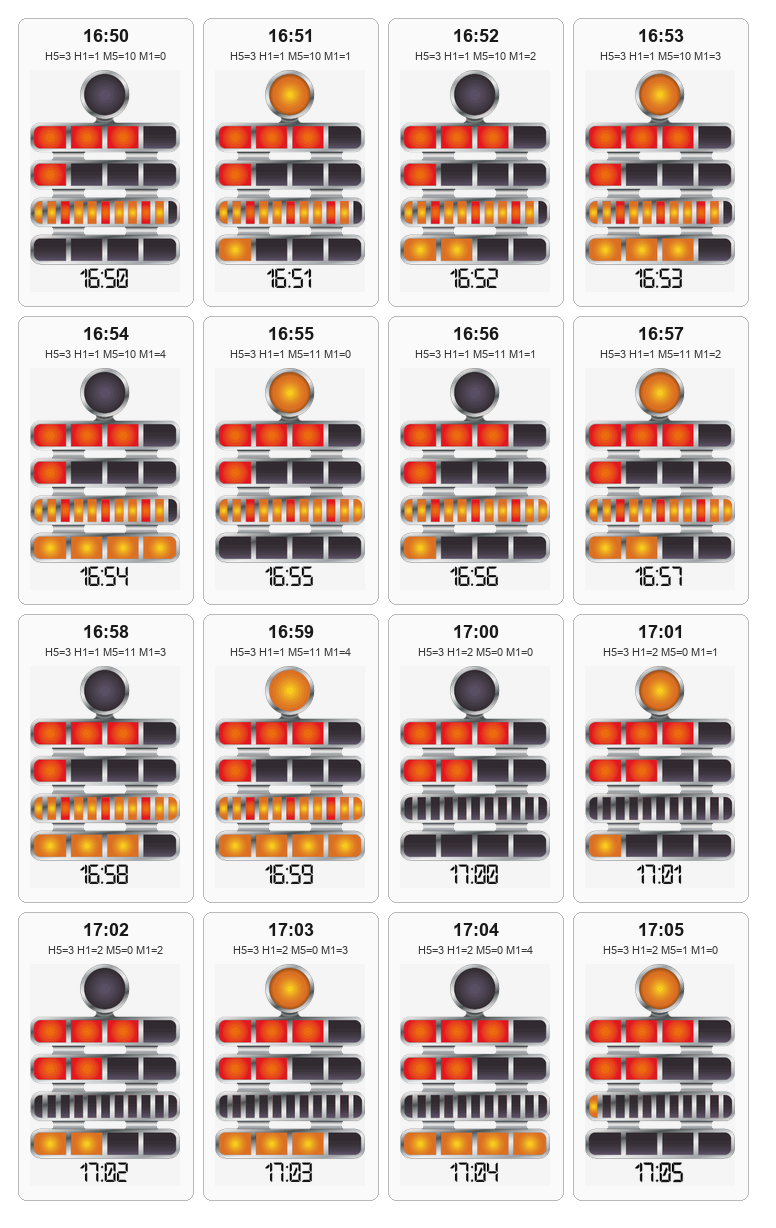
\includegraphics[height=0.74\textheight,keepaspectratio]{berlin_uhr_sequence_1650_1705.png}
\caption{Minute-by-minute Berlin-Uhr sequence from 16:50 through 17:05, extracted and labeled from a Commons animation \cite{commonsBerlinUhrGif}. Each panel gives the row decomposition $H_5=\lfloor H/5\rfloor$, $H_1=H\bmod 5$, $M_5=\lfloor M/5\rfloor$, and $M_1=M\bmod 5$.}
\label{fig:berlinUhrSequence}
\end{figure}

The Berlin-Uhr sequence in \autoref{fig:berlinUhrSequence} shows why the modular formulation is not arbitrary. The clock does not display time by rotating hands; it displays a quotient-and-remainder decomposition. The hour is split into five-hour blocks plus a one-hour remainder, and the minute is split into five-minute blocks plus a one-minute remainder:
\begin{equation}
    H = 5H_5 + H_1,\qquad M = 5M_5 + M_1.
\end{equation}
Across the sequence, $M_1$ cycles through $0,1,2,3,4$ and then resets while $M_5$ increments. At 17:00, the minute rows reset and $H_1$ increments from $1$ to $2$. The top seconds lamp adds a parity layer, toggling by $S \bmod 2$. This makes the Berlin-Uhr a legitimate mechanism analogy for Kryptos research: it is a public Berlin clock whose visible state is already modular, row-based, and mask-like.

The modular view also clarifies how distance metrics enter the PRO workflow. Let $\Delta_{\alpha}(c,p)$ denote the vector of modular differences $\alpha(c_i)-\alpha(p_i) \bmod 26$ over a span. For a candidate method with predicted residue vector $\widehat{\Delta}$, the crib-level modular error can be written as
\begin{equation}
    d_H\!\left(\Delta_{\alpha}(\Cipher_4,\Plain_4),\widehat{\Delta}\right),
\end{equation}
where $d_H$ is Hamming distance. Candidate plaintexts can also be compared by edit distance or word-skeleton distance, but those linguistic distances are secondary. The modular residue test is the harder cryptanalytic filter because it ties the candidate back to the actual ciphertext.

\section{Paired Research Optimization}
Paired Research Optimization is a constraint-ranking procedure. It is not a cipher. It does not derive plaintext from ciphertext. Its purpose is to expose which plaintext hypotheses deserve further cryptanalytic testing and which should be discarded before method search begins.

The procedure has six stages:
\begin{enumerate}
    \item normalize each candidate phrase and reject any phrase whose normalized length is not 97;
    \item reject any \Kfour\ phrase that fails either public crib span;
    \item compute the modular residue vectors implied by the public crib spans under each alphabet being tested;
    \item segment each phrase into words and compute word intervals in normalized character coordinates;
    \item reward same-position structural alignment between \Kfour\ and \Kfive, especially where shared words occupy identical intervals;
    \item penalize unsupported claims, including any claim that a plausible phrase is a solved decryption without an explicit method.
\end{enumerate}

For a phrase $p$ with words $w_1,\ldots,w_m$, define the word interval function
\begin{equation}
    I_j(p) =
    \left[
    1 + \sum_{r<j} |\Norm(w_r)|,\,
    \sum_{r\leq j} |\Norm(w_r)|
    \right].
\end{equation}
The word-length skeleton is
\begin{equation}
    \mathbf{s}(p) =
    \bigl(|\Norm(w_1)|,\ldots,|\Norm(w_m)|\bigr).
\end{equation}
Let $\WordSet(P_4)$ denote the set of normalized word intervals induced by $P_4$. A shared-word interval is an interval $I=[a,b]$ for which the same normalized word occupies the same character interval in both members of the pair. The weak existence condition is
\begin{equation}
    \exists S \subseteq \WordSet(P_4):
    \quad
    P_5[I] = P_4[I]\ \text{for each shared word interval } I \in S.
\end{equation}
The equivalent quantified final form is
\begin{equation}
    \exists S \subseteq \WordSet(P_4): \forall I \in S,\quad P_5[I] = P_4[I].
\end{equation}
When the companion is written as a synthetic \Kfive\ proposal, the same constraint is
\begin{equation}
    \exists S \subseteq \WordSet(P_4): \forall I \in S,\quad Q_5[I] = P_4[I].
\end{equation}
The strictest paired condition considered in this paper is
\begin{equation}
    \mathbf{s}(p_4)=\mathbf{s}(p_5).
\end{equation}
This is stronger than Sanborn's public statement. The statement concerns same-position coded words, not necessarily identical plaintext word skeletons. PRO uses skeleton equality as a heuristic proxy because it produces falsifiable, auditable candidate pairs.

\section{Scoring Model}
The PRO objective can be written as a paired optimization problem:
\begin{equation}
\begin{aligned}
    (P_4^\star,Q_5^\star)
    \in
    \ArgMax_{P_4,Q_5}
    \Big[
    &\operatorname{English}(P_4)
    + \operatorname{English}(Q_5) \\
    &+ \lambda_1 \operatorname{Cribs}(P_4)
    + \lambda_2 \operatorname{SameWordIntervals}(P_4,Q_5) \\
    &+ \lambda_3 \operatorname{K2BuriedTheme}(Q_5)
    + \lambda_4 \operatorname{EgyptWallClockTheme}(P_4)
    \Big],
\end{aligned}
\end{equation}
Here $\lambda_1,\ldots,\lambda_4 \geq 0$ are research weights. The crib term is effectively a hard gate for \Kfour. The same-word term implements the interval condition above. The buried-theme term scores the cache/site relation announced for \Kfive. The Egypt-wall-clock term scores the Egypt, Berlin Wall, and Berlin World Clock constraints announced for \Kfour.

For implementation, each pair also receives a heuristic decomposition
\begin{equation}
    \Score(p_4,p_5)
    =
    \Score_{\mathrm{crib}}
    + \Score_{\mathrm{length}}
    + \Score_{\mathrm{mod}}
    + \Score_{\mathrm{skeleton}}
    + \Score_{\mathrm{theme}}
    + \Score_{\mathrm{culture}}
    + \Score_{\mathrm{geo}}
    + \Score_{\mathrm{style}}
    - \Score_{\mathrm{penalty}}.
\end{equation}
The crib and length components are hard filters. If a \Kfour\ candidate fails either public crib or if either phrase fails the 97-character requirement, the pair is rejected rather than merely down-ranked. The modular component rewards compatibility with residue vectors produced by an independently specified method. A candidate phrase can pass the language filters and still receive no modular credit if no ciphertext-to-plaintext mechanism accounts for the crib residues.

The skeleton component rewards identical word-length structure and same-position shared words. The thematic component rewards explicit coverage of the Sanborn clues: Egypt, Berlin Wall, Berlin World Clock, delivery of a message, and the \Ktwo/\Kfive\ buried-site theme. The cultural component rewards historically coherent use of Egypt, Berlin, Cold War imagery, and Kryptos's message-delivery frame. The geographic component rewards consistency with Alexanderplatz, the Berlin-Uhr background, and the CIA/Langley grounds clues. The style component rewards compactness, ordinary English syntax, and consistency with the terse, clue-like character of prior Kryptos plaintexts. The penalty term is essential: a pair loses credit if it is too self-referential, forces unsupported symbolism, depends on private evidence, or implies that a plaintext guess is equivalent to a cipher solution.

The score is not a probability. It is a triage device. Its value is in making research judgments explicit enough that another researcher can adjust weights, add constraints, or reject a candidate without changing the entire framework.

\section{Top Candidate Pair}
The highest-ranked pair from the PRO discussion is:
\begin{table}[H]
\caption{Top PRO candidate pair. The phrases are hypotheses, not decryptions.}
\centering
\small
\begin{tabular}{L{0.12\textwidth}L{0.74\textwidth}}
\toprule
Message & Candidate plaintext \\
\midrule
\Kfour &
EGYPT TRIP MESSAGE HIDES EAST NORTHEAST PAST A FALLEN WALL WHERE WORLD TIME BERLIN CLOCK DELIVERS THE FINAL MESSAGE \\
\Kfive &
CACHE LIES MESSAGE HIDES SITE SOMEWHERE PAST A BURIED WALL WHERE STONE TIME COPPER FIELD DELIVERS THE FINAL MESSAGE \\
\bottomrule
\end{tabular}
\end{table}

In the discussion table, this pair was scored at 94/100. This paper keeps the same ranking but labels the rows as decryption hypotheses rather than completed decryptions.

Both phrases normalize to 97 letters. The \Kfour\ phrase satisfies the public cribs exactly:
\begin{equation}
    \Norm(p_4)[22:34] = \texttt{EASTNORTHEAST},
\end{equation}
and
\begin{equation}
    \Norm(p_4)[64:74] = \texttt{BERLINCLOCK}.
\end{equation}
The \Kfive\ phrase deliberately does not force those same plaintext cribs. Instead, it places companion semantic material in the corresponding intervals:
\begin{equation}
    \Norm(p_5)[22:34] = \texttt{SITESOMEWHERE},
\end{equation}
and
\begin{equation}
    \Norm(p_5)[64:74] = \texttt{COPPERFIELD}.
\end{equation}
This reflects the paper's interpretation of \Kfive\ as a future companion clue rather than a second copy of \Kfour.

The word interval alignment is shown in \autoref{tab:sharedIntervals}. The pair shares a substantial same-position scaffold while allowing the middle clue-bearing spans to diverge.

\begin{table}[H]
\caption{Same-position shared words in the top candidate pair.}
\label{tab:sharedIntervals}
\centering
\small
\begin{tabular}{L{0.32\textwidth}C{0.16\textwidth}C{0.16\textwidth}}
\toprule
Shared word & Start & End \\
\midrule
MESSAGE & 10 & 16 \\
HIDES & 17 & 21 \\
PAST & 35 & 38 \\
A & 39 & 39 \\
WALL & 46 & 49 \\
WHERE & 50 & 54 \\
TIME & 60 & 63 \\
DELIVERS & 75 & 82 \\
THE & 83 & 85 \\
FINAL & 86 & 90 \\
MESSAGE & 91 & 97 \\
\bottomrule
\end{tabular}
\end{table}

The pair earns a high heuristic score because it captures the public \Kfour\ clue set while giving \Kfive\ a coherent buried-site analogue. The first phrase connects Egypt, a fallen wall, world time, the Berlin clock, and delivery of a message. The second phrase maps the same grammatical structure onto cache, site, buried wall, copper field, and final message language.

\begin{table}[H]
\caption{Scored decryption hypotheses from the PRO discussion. Scores rank research usefulness, not proof of solution.}
\label{tab:scoredHypotheses}
\centering
\tiny
\setlength{\tabcolsep}{2pt}
\begin{tabular}{C{0.08\textwidth}L{0.41\textwidth}L{0.41\textwidth}C{0.06\textwidth}}
\toprule
Pair & \Kfour\ hypothesis & \Kfive\ companion hypothesis & Score \\
\midrule
A &
EGYPT TRIP MESSAGE HIDES EAST NORTHEAST PAST A FALLEN WALL WHERE WORLD TIME BERLIN CLOCK DELIVERS THE FINAL MESSAGE &
CACHE LIES MESSAGE HIDES SITE SOMEWHERE PAST A BURIED WALL WHERE STONE TIME COPPER FIELD DELIVERS THE FINAL MESSAGE &
94 \\
B &
A KRYPTOS CIPHER MESSAGE EAST NORTHEAST WHERE EGYPT WALL AND WORLD TIME MET BERLIN CLOCK DELIVERS THE FINAL MESSAGE &
A KRYPTOS CIPHER MESSAGE EAST NORTHEAST WHERE EARTH MAGNETIC FIELD POINTS BERLIN CLOCK SHOWS WHERE CACHE IS BURIED &
92 \\
C &
MY HIDDEN CIPHER MESSAGE EAST NORTHEAST WHERE EGYPT WALL AND WORLD TIME MET BERLIN CLOCK SHOWS WHERE HIDDEN PLACE IS &
MY HIDDEN CIPHER MESSAGE EAST NORTHEAST WHERE EARTH MAGNETIC FIELD POINTS BERLIN CLOCK SHOWS WHERE CACHE IS BURIED &
90 \\
D &
COUNT LIGHT FIELDS TO USE EAST NORTHEAST LIGHT FIELDS GIVE THE HIDDEN ROUTE BERLIN CLOCK DELIVERS THE FINAL MESSAGE &
COUNT LIGHT FIELDS TO USE EAST NORTHEAST LIGHT FIELDS MARK THE BURIED CACHE BERLIN CLOCK SHOWS WHERE CACHE IS BURIED &
84 \\
\bottomrule
\end{tabular}
\end{table}

The score column is not a probability estimate and should not be read as confidence that a phrase is true. It is a reproducibility aid: higher-scored rows preserve more public constraints and therefore deserve earlier method search, while lower-scored rows remain useful as structured alternatives.

The scored table preserves the working discussion's main distinction. Pair A has the best balance of public crib compliance, cultural fit, and \Kfive\ companion structure. Pair B and Pair C are stronger skeleton matches but more self-referential. Pair D is mechanistically interesting because ``light fields'' echoes the Berlin-Uhr, but it is semantically weaker after Sanborn's World Clock clarification.

\section{Secondary Candidate Analysis}
The lower-ranked candidates are not discarded. They encode distinct hypotheses about how literal, self-referential, or mechanical the final message may be. This paper therefore treats them as alternate decryption hypotheses with explicit acceptance and rejection conditions.

\subsection{Pair B: Self-Referential Kryptos Cipher}
Pair B is:
\begin{quote}
\footnotesize\raggedright
\textbf{\Kfour:}\\
A KRYPTOS CIPHER MESSAGE EAST NORTHEAST WHERE EGYPT WALL AND WORLD TIME MET BERLIN CLOCK DELIVERS THE FINAL MESSAGE

\textbf{\Kfive:}\\
A KRYPTOS CIPHER MESSAGE EAST NORTHEAST WHERE EARTH MAGNETIC FIELD POINTS BERLIN CLOCK SHOWS WHERE CACHE IS BURIED
\end{quote}
This pair has high structural value because both candidates normalize to 97 letters and share a strong opening scaffold: \texttt{A KRYPTOS CIPHER MESSAGE}. It directly identifies the object as a Kryptos message, preserves the released \Kfour\ cribs, and makes the \Kfive\ companion explicitly echo \Ktwo\ through earth, magnetic field, cache, and buried language.

The acceptance case for Pair B is strongest if authenticated plaintext confirms that \Kfour\ is explicitly self-referential. It would also gain support if a recovered method shows that the opening positions encode a phrase equivalent to \texttt{AKRYPTOSCIPHERMESSAGE}, or if \Kfive\ is later shown to repeat the same self-labeling structure. Pair B should be rejected if the authenticated text avoids direct reference to Kryptos, if the opening interval is historically descriptive rather than self-labeling, or if the phrase ``where Egypt wall and world time met'' proves too compressed to match Sanborn's intended language.

\subsection{Pair C: Hidden-Message Form}
Pair C is:
\begin{quote}
\footnotesize\raggedright
\textbf{\Kfour:}\\
MY HIDDEN CIPHER MESSAGE EAST NORTHEAST WHERE EGYPT WALL AND WORLD TIME MET BERLIN CLOCK SHOWS WHERE HIDDEN PLACE IS

\textbf{\Kfive:}\\
MY HIDDEN CIPHER MESSAGE EAST NORTHEAST WHERE EARTH MAGNETIC FIELD POINTS BERLIN CLOCK SHOWS WHERE CACHE IS BURIED
\end{quote}
This pair is valuable because it reduces the overt \texttt{KRYPTOS} self-reference while retaining a tight same-position structure. The phrase \texttt{MY HIDDEN CIPHER MESSAGE} is compatible with the meaning of Kryptos as hidden and with the sculpture's message-delivery theme. It also gives both members of the pair a clear end function: the clock shows where something hidden or buried is.

The acceptance case for Pair C is strongest if the authenticated \Kfour\ plaintext uses first-person or artist-centered phrasing, such as ``my hidden'' or an equivalent authorial voice. It also becomes stronger if \Kfive\ later proves to keep the same opening language while changing the object from hidden place to buried cache. Pair C should be rejected if the true \Kfour\ text is impersonal, if the final clause does not involve showing or locating, or if the ``my'' construction conflicts with Sanborn's documented plaintext style.

\subsection{Pair D: Light-Field Mechanism Candidate}
Pair D is:
\begin{quote}
\footnotesize\raggedright
\textbf{\Kfour:}\\
COUNT LIGHT FIELDS TO USE EAST NORTHEAST LIGHT FIELDS GIVE THE HIDDEN ROUTE BERLIN CLOCK DELIVERS THE FINAL MESSAGE

\textbf{\Kfive:}\\
COUNT LIGHT FIELDS TO USE EAST NORTHEAST LIGHT FIELDS MARK THE BURIED CACHE BERLIN CLOCK SHOWS WHERE CACHE IS BURIED
\end{quote}
This pair has lower semantic confidence but high mechanism value. Unlike Pairs B and C, it makes the Berlin-Uhr hypothesis explicit through \texttt{COUNT LIGHT FIELDS}. That phrase maps naturally onto the set-theory clock's illuminated rows and additive field-counting principle \cite{berlinUhrOfficial}. It is therefore the best candidate if the word \texttt{BERLINCLOCK} is not only a semantic pointer to the World Clock but also a hidden instruction to count or index clock fields.

The acceptance case for Pair D is strongest if a reproducible method uses light-field counts, binary masks, row totals, or clock-field positions to generate the modular residues in \autoref{tab:modularResidues}. It would also gain support if the authenticated text contains action verbs such as count, use, mark, give, or route. Pair D should be rejected if Sanborn's World Clock clue is purely semantic, if no light-field procedure reproduces the released crib residues, or if the true plaintext does not contain procedural language.

\subsection{Cross-Candidate Value}
The candidates are useful even when rejected because each isolates a different explanatory axis. Pair B tests direct self-reference. Pair C tests hidden-message authorship without naming Kryptos. Pair D tests a mechanical clock-field reading. Pair A remains the lead because it balances all axes, but the secondary candidates define the neighboring hypothesis space. A future solution should not merely select a phrase; it should explain why these nearby alternatives fail.

\section{Why the Pair Is Plausible}
The top pair is plausible for three reasons. First, it respects the hard constraints. The \Kfour\ phrase has exactly 97 normalized letters and contains both released plaintext spans in the required positions. Second, it gives the new 2025 clues functional roles rather than treating them as isolated keywords. Egypt appears as the opening provenance cue; the fall of the Berlin Wall appears as ``fallen wall''; the Berlin World Clock appears through the contiguous crib; and the phrase ``delivers the final message'' implements Sanborn's message-delivery clue.

Third, the \Kfive\ phrase uses the same skeleton to convert the public \Kfour\ semantics into a buried-site hypothesis. In this reading, \Kfour\ points outward through public historical and geographic references, while \Kfive\ points inward toward an object, cache, field, or site. That division is consistent with the public claim that \Kfive\ is connected to the \Ktwo\ buried-language motif \cite{verganoFinalClues2025}.

The pair also avoids a common overfitting pattern. It does not assume that \Kfive\ must repeat \texttt{EASTNORTHEAST} or \texttt{BERLINCLOCK} as plaintext. Since the public clue concerns shared coded words, the safer research posture is to allow corresponding plaintext spans to diverge unless a future \Kfive\ ciphertext proves otherwise.

\section{Why the Pair Is Not a Solution}
The same pair is not a solution for equally important reasons. It has no enciphering method. It does not explain how the public \Kfour\ ciphertext maps to the proposed plaintext. It does not recover a key, tableau path, transposition, null system, matrix operation, or mixed procedure. It only satisfies visible language constraints.

This distinction matters because recent public reporting separates possession of plaintext from knowledge of method. Scientific American reported that the archival discovery exposed plaintext scraps, while also emphasizing that method and creative context remain separate from the words alone \cite{basilioKryptosSolution2025}. The Associated Press similarly reported Sanborn's distinction between discovering text and deciphering it by method \cite{caseyAP2025}.

Therefore the top pair should be treated as a target for method search. A future cryptanalytic argument would need to specify a reproducible transformation from the public ciphertext
\begin{quote}
\small\ttfamily
OBKRUOXOGHULBSOLIFBBWFLRVQQPRNGKSS\\
OTWTQSJQSSEKZZWATJKLUDIAWINFBNYPVTTMZFPK\\
WGDKZXTJCDIGKUHUAUEKCAR
\end{quote}
to the proposed \Kfour\ plaintext. Without that transformation, the candidate remains a structured hypothesis.

\section{Berlin Clock Backgrounds and Mechanism Search}
The \texttt{BERLINCLOCK} clue has two relevant Berlin-clock backgrounds. The first is the Berlin-Uhr, also called the set-theory clock. It was commissioned by the Berlin Senate in 1975, designed by Dieter Binninger, and originally located at Kurfürstendamm on the corner with Uhlandstraße. After decommissioning in 1995, it was given a new home in Budapester Straße in front of the Europa-Center in 1996 \cite{europaCenterSetTheoryClockArchive}. Its display encodes time by illuminated fields: rows of lights represent five-hour, one-hour, five-minute, and one-minute quantities, and the time is read by adding the lit fields \cite{berlinUhrOfficial}. This makes it cryptanalytically attractive because it is already a modular, row-structured, light-field encoding device.

The second is the Urania World Clock on Alexanderplatz. Berlin's official city portal describes it as a DDR-era installation opened in 1969, designed by Erich John, built around a 24-sided rotating cylinder representing the Earth's time zones, and located at Alexanderplatz \cite{berlinWorldClock}. Sanborn's 2025 clue identifies this World Clock as the referent of \texttt{BERLINCLOCK} \cite{verganoFinalClues2025}. That makes the World Clock the stronger semantic background for plaintext interpretation.

\begin{figure}[H]
\centering
\begin{subfigure}[t]{0.36\textwidth}
\centering
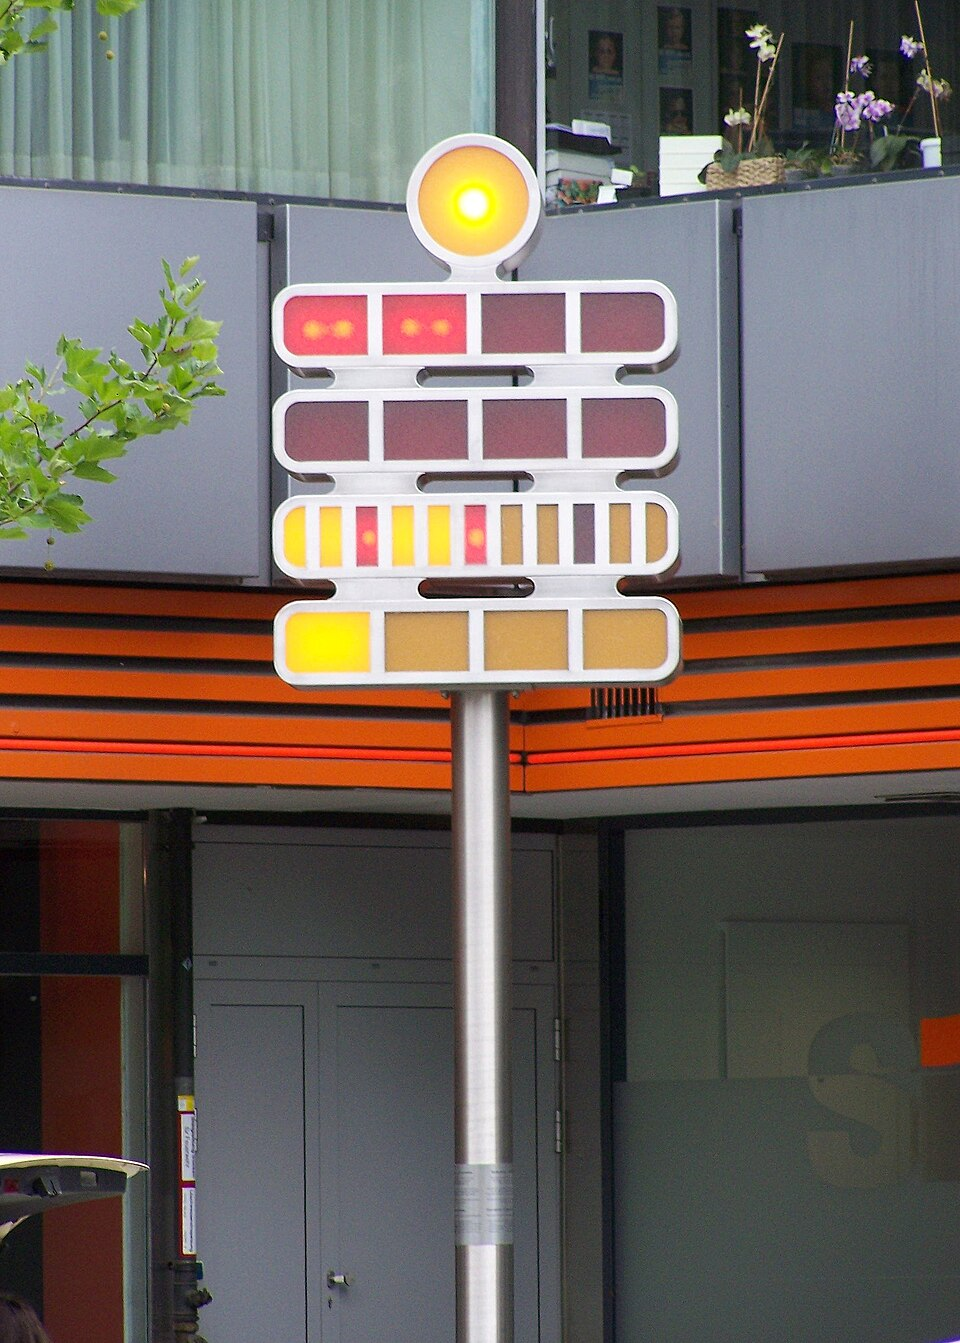
\includegraphics[width=\textwidth,height=0.30\textheight,keepaspectratio]{mengenlehreuhr_berlin_uhr.jpg}
\caption{Berlin-Uhr near the Europa-Center.}
\end{subfigure}
\hfill
\begin{subfigure}[t]{0.56\textwidth}
\centering
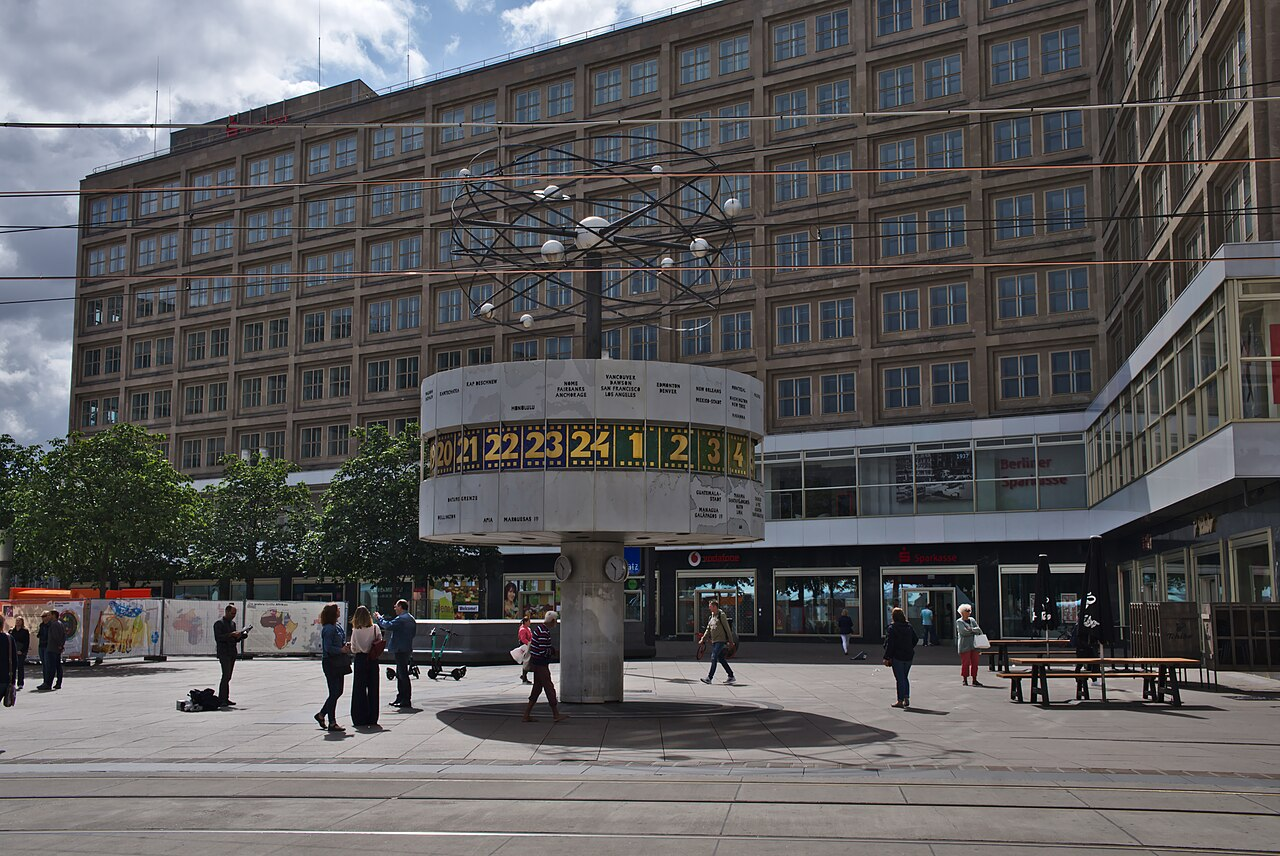
\includegraphics[width=\textwidth,height=0.30\textheight,keepaspectratio]{alexanderplatz_urania_world_clock.jpg}
\caption{Urania World Clock at Alexanderplatz.}
\end{subfigure}
\caption{The two Berlin clock backgrounds used in this paper. The Berlin-Uhr supplies a modular light-field mechanism, while the Urania World Clock supplies the Sanborn-identified semantic referent for \texttt{BERLINCLOCK} \cite{commonsMengenlehreuhrPhoto,commonsAlexanderplatzWorldClockPhoto}.}
\label{fig:berlinClockPhotos}
\end{figure}

\begin{figure}[H]
\centering
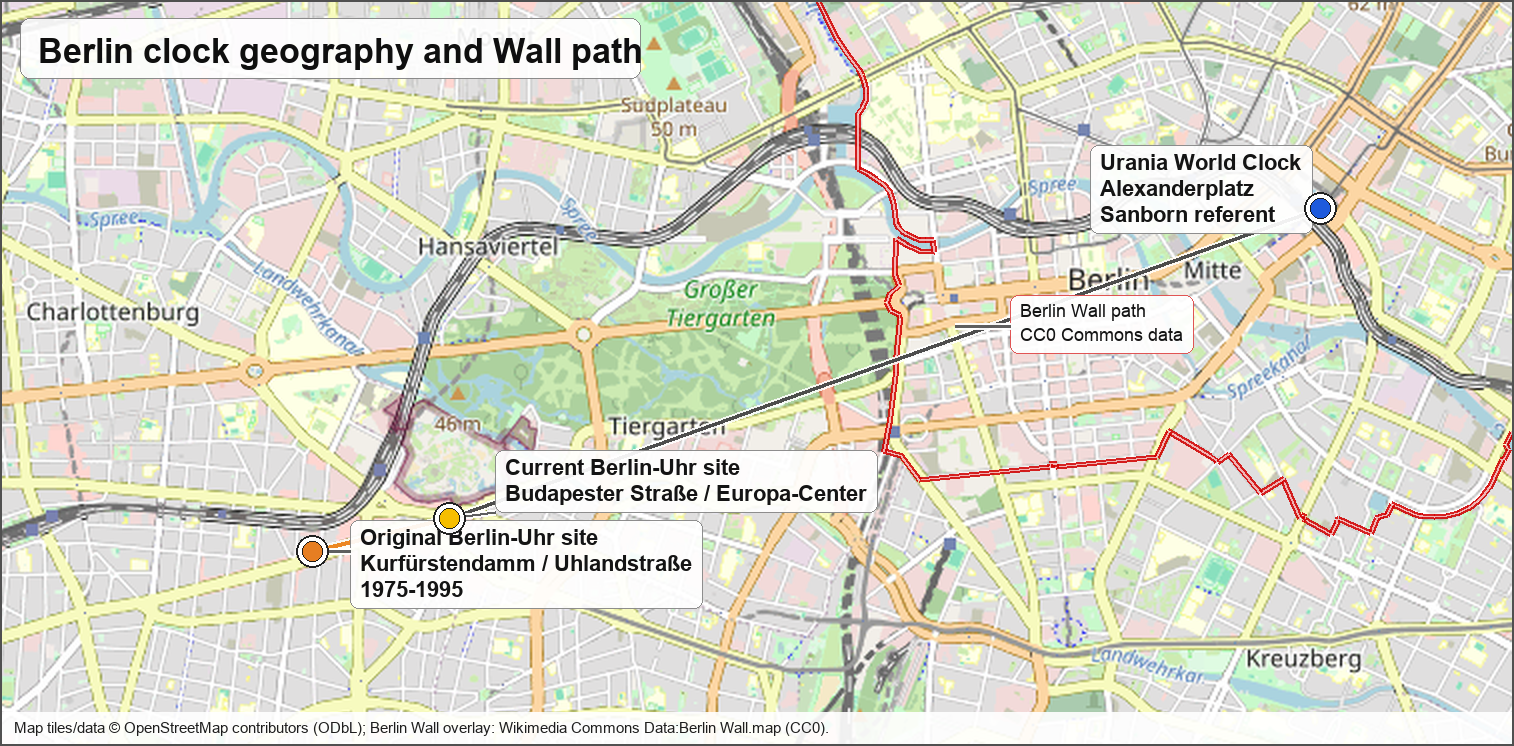
\includegraphics[width=\textwidth]{berlin_clock_geography_map.png}
\caption{Berlin map of the clock clues. The Berlin-Uhr contributes the modular mechanism analogy and has both an original Kurfürstendamm/Uhlandstraße site and a current Budapester Straße/Europa-Center site; the Urania World Clock at Alexanderplatz remains the Sanborn-identified semantic referent for \texttt{BERLINCLOCK}. The basemap uses OpenStreetMap tiles, and the Berlin Wall overlay uses the CC0 Commons \textit{Data:Berlin Wall.map} path \cite{europaCenterSetTheoryClockArchive,berlinWorldClock,openStreetMapTiles,commonsBerlinWallMap}.}
\label{fig:geographicMap}
\end{figure}

Both clocks remain relevant, but for different reasons. The World Clock is relevant because Sanborn explicitly tied it to the released plaintext span. It supports language involving world time, Berlin, public space, time zones, historical Berlin, and the fall of the Wall. The set-theory clock is relevant because it supplies a mechanism-shaped object: a row/field representation that naturally suggests modular residues, binary masks, cyclic offsets, and row-column extraction. In other words, the World Clock should dominate semantic reading, while the set-theory clock remains a possible mechanical analogy that must earn its place by reproducing the modular crib profiles in \autoref{tab:modularResidues}.

PRO therefore separates semantic and mechanical uses of clocks. As a semantic constraint, \texttt{BERLINCLOCK} should be interpreted through the World Clock clue. As a mechanism hypothesis, either clock background may be tested only if it produces an explicit mapping from ciphertext to plaintext and satisfies all released cribs. Examples include cyclic rotations, modular offsets, radial readings, row-column clocks, binary light masks, and time-zone indexed permutations. None of those mechanisms is assumed in the candidate pair.

This separation prevents clue drift. A single word such as ``clock'' can inspire dozens of mechanisms, but only a reproducible mechanism can validate a plaintext. PRO uses the World Clock clue to guide candidate language, uses the set-theory clock to motivate modular tests, and keeps both subordinate to ciphertext-derived verification.

\section{Falsification Conditions}
A useful Kryptos hypothesis should be easy to reject. Any scored pair would be falsified under one or more of the following conditions:
\begin{enumerate}
    \item a public release of the authenticated \Kfour\ plaintext conflicts with any normalized character in that pair's proposed \Kfour\ phrase;
    \item a public release of \Kfive\ shows that its length, same-position shared words, or thematic relation differs from that pair's assumptions;
    \item a valid public enciphering method maps $\Cipher_4$ to a different 97-character plaintext;
    \item independent testing shows that the candidate phrase family was selected by unconstrained thematic fitting rather than by constraints strong enough to reduce the search space meaningfully;
    \item the phrase cannot be reconciled with authenticated Sanborn notes, tableaux, or stated creative context;
    \item a candidate's distinctive axis fails. For Pair B, that axis is self-reference. For Pair C, it is authorial hidden-message language. For Pair D, it is a light-field clock mechanism.
\end{enumerate}

These failure conditions are not weaknesses. They are the reason to frame the result as research rather than revelation. A candidate pair that cannot be falsified is not useful for cryptanalysis.

\section{Future Work}
The next stage is method search. The candidate pair suggests several testable directions without endorsing any of them: direct substitution under the Kryptos alphabet, layered Vigenere variants, transposition after keyed substitution, null extraction, row-column matrix readings, clock-indexed permutations, and mixed systems involving the sculpture's physical layout. Each proposed method should be evaluated against all 24 released \Kfour\ plaintext characters before being evaluated against the remaining unknown positions.

A second direction is corpus discipline. Candidate plaintext generation should use a fixed vocabulary derived from public Kryptos sources, Sanborn clues, solved \Kone--\Kthree\ themes, and the announced \Kfive\ relation. This would reduce the risk of unconstrained phrase-fitting. A third direction is interval ablation: remove one thematic constraint at a time and measure how many 97-character skeletons remain. If a constraint does not reduce the space, it should carry little scoring weight.

Finally, any AI-assisted workflow should log rejected candidates as carefully as accepted candidates. Kryptos research has suffered from repeated rediscovery of attractive but non-methodological guesses. A reproducible negative record would make future work more efficient.

\section{Conclusion}
This paper reformulated PRO as a constraint-based research framework for Kryptos \Kfour\ and the announced \Kfive. The central result is a method, not a decryption. PRO generates paired candidate plaintexts by enforcing exact \Kfour\ crib positions, 97-character length, modular residue compatibility, word-skeleton alignment, shared-word interval notation, thematic consistency with public Sanborn clues, and an explicit separation between plausible plaintext and demonstrated cipher method.

The top candidate pair is useful because it turns scattered public evidence into a concrete, testable research object. It is also limited: without a method that maps the public \Kfour\ ciphertext to the proposed text, it cannot be called a solution. That boundary is the paper's main methodological point. In the current public state of Kryptos, disciplined hypothesis generation is valuable only when it remains subordinate to reproducible cryptanalysis.

\begin{theappendices}
\setcounter{section}{0}
\renewcommand{\thesection}{Appendix \Alph{section}}
\section{Reproducibility Audit}
This appendix records the mechanical checks used to verify the candidate table and the modular arithmetic claims. The source distribution includes a Python audit script. Running that script prints \texttt{Appendix A audit passed} when all checks below hold.

\begin{table}[H]
\caption{Appendix A audit targets. These checks verify structure only; they do not validate a cipher method.}
\label{tab:appendixAudit}
\centering
\small
\begin{tabular}{L{0.40\textwidth}L{0.44\textwidth}}
\toprule
Check & Expected result \\
\midrule
All scored pairs A--D & $\Len(\Norm(P_4))=97$ and $\Len(\Norm(Q_5))=97$ \\
All scored \Kfour\ candidates & $\Norm(P_4)[22:34]=\texttt{EASTNORTHEAST}$ \\
All scored \Kfour\ candidates & $\Norm(P_4)[64:74]=\texttt{BERLINCLOCK}$ \\
Top-pair companion spans & $\Norm(Q_5)[22:34]=\texttt{SITESOMEWHERE}$ and $\Norm(Q_5)[64:74]=\texttt{COPPERFIELD}$ \\
A--Z residues & \texttt{BLZCDCYYGCKAZ} and \texttt{MUYKLGKORNA} \\
Kryptos-alphabet residues & \texttt{RDUMRIYWOYNKY} and \texttt{ELYOIECBAQK} \\
Top-pair shared intervals & 11 intervals: MESSAGE, HIDES, PAST, A, WALL, WHERE, TIME, DELIVERS, THE, FINAL, MESSAGE \\
\bottomrule
\end{tabular}
\end{table}

The audit procedure is:
\begin{enumerate}
    \item normalize each phrase by deleting every nonalphabetic character and uppercasing the result;
    \item assert 97 normalized characters for each \Kfour\ and \Kfive\ phrase in \autoref{tab:scoredHypotheses};
    \item assert the two public \Kfour\ crib intervals in every scored \Kfour\ phrase;
    \item compute the standard-alphabet and Kryptos-alphabet modular residues using $\alpha(c_i)-\alpha(p_i)\bmod 26$;
    \item segment the top pair into normalized word intervals and assert the shared intervals in \autoref{tab:sharedIntervals}.
\end{enumerate}

The audit is intentionally narrow. It verifies that the paper's tables, residue strings, and interval statements are internally reproducible. It does not test any enciphering method, and it does not convert any candidate phrase into a solution.
\end{theappendices}

\buildBibliography
\end{thesisbody}

\end{document}
